%!TEX root = ./main.tex

\chapter{Ports details}

\section{Posix}

\subsection{Overview}

\subsection{Monocore}

\subsection{Multicore}

\section{PowerPC}
\label{sec:ppcport}
\subsection{System services} \label{sec:systemservices}

The PowerPC port uses the \asfct{sc} software interrupt to call system services \cite{mpc32bsc}. \asfct{sc} stands for System Call. It saves the current \reg{PC} in \reg{SRR0} register and the current \reg{MSR} in \reg{SRR1} register and jump to the System Call handler.

The id of the system service to call is given in the \reg{r0} register and \reg{r0} save and restore are added around. For instance, the following listing gives the \api{ActivateTask} service code. These function are generated from templates by goil (see \ref{sec:generatedfiles}) and are part of the {\em invoque} layer (see \ref{sec:invoque}):

\begin{lstlisting}[language=C]
  .global ActivateTask
ActivateTask:
  subi r1,r1,4                       /* make room on stack    */
  stw  r0,0(r1)                      /* save r0               */
  li   r0,OSServiceId_ActivateTask   /* load r0 with the id   */
  sc                                 /* system call           */
  lwz  r0,0(r1)                      /* restore r0            */
  addi r1,r1,4                       /* restore stack         */
  blr                                /* return                */
  
  .type ActivateTask,@function
  .size ActivateTask,$$-ActivateTask
\end{lstlisting}

When the System Call begin execution, the process stack has the mapping depicted in figure \ref{fig:stackbeginningSC}.

\begin{figure}[htbp] %  figure placement: here, top, bottom, or page
\begin{minipage}{0.5\textwidth}
    \centering
  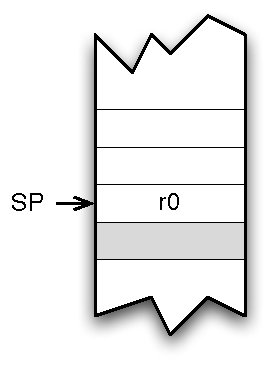
\includegraphics[scale=.6]{pictures/PStackAfterInvoque} 
\end{minipage}
\begin{minipage}{0.5\textwidth}
   \caption{Process stack mapping at the beginning of the System Call handler. The grayed zone represents an unknown content depending on from where the service was called.}\label{fig:stackbeginningSC}
\end{minipage}
\end{figure}

\subsection{Dispatching the service call}

The System Call handler is usually located in the \hex{0C00} exception handler but, depending on the CPU kind, it may be located elsewhere. Since the available memory for the interrupt or exception handler may vary, a jump is made to the \cfunction{tpl_sc_handler}.%:

%\begin{lstlisting}
%  .section  .SC_vector  CODE_ACCESS_RIGHT
%tpl_sc_vector:
%  b   tpl_sc_handler
%
%  .section  .SC_handler CODE_ACCESS_RIGHT
%\end{lstlisting}

\cfunction{tpl_sc_handler} performs the following tasks:
\begin{penum}
\item saves additional registers to be able to work
\item disables memory protection
\item switches to kernel stack if needed
\item calls the service
\item performs a context switch if needed and programs the MPU.
\item switches back to the process stack if needed
\item enable memory protection
\item restore registers
\item get back to the process
\end{penum}

\note{Currently the PowerPC port does not support tasks that use floating point registers}

\subsubsection{Saving additional registers}

The following registers are saved: \var{lr}, \var{cr}, \var{r11} and \var{r12}. In fact, it should be not necessary to save \var{r11} and \var{r12} because these registers are volatile as defined in the PowerPC EABI \cite{PPCeabi} but we prefer a conservative approach. Register saving is done by the following code at start of the \cfunction{tpl_sc_handler} and the mapping of the process stack is depicted at figure \ref{fig:stackSavingSC}:

\begin{lstlisting}[language=C]
  subi  r1,r1,PS_FOOTPRINT  /* Make room on stack */

  stw   r11,PS_R11(r1)      /* Save r11           */
  stw   r12,PS_R12(r1)      /* Save r12           */
  mflr  r11
  stw   r11,PS_LR(r1)       /* Save lr            */
  mfcr  r11
  stw   r11,PS_CR(r1)       /* Save cr            */
\end{lstlisting}

\begin{figure}[htbp] %  figure placement: here, top, bottom, or page
\begin{minipage}{0.5\textwidth}
    \centering
  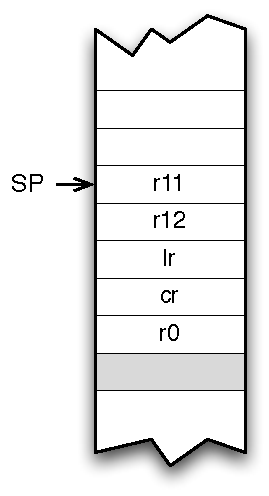
\includegraphics[scale=.6]{pictures/PStackAfterSCSaving} 
\end{minipage}
\begin{minipage}{0.5\textwidth}
   \caption{Process stack mapping after additional registers have been saved by the beginning of the System Call handler.}\label{fig:stackSavingSC}
\end{minipage}
\end{figure}

\subsubsection{Disabling memory protection}

This part of the dispatch layer is done in the \cfunction{tpl_enter_kernel} function and is assembled only if \cmacro{WITH_MEMORY_PROTECTION} is set to \YES. After saving the \reg{lr}, the \cfunction{tpl_kernel_mp} function is called and does the actual job. At last \reg{lr} is restored.

\begin{lstlisting}[language=C]
#if WITH_MEMORY_PROTECTION == YES
  /*
   * Switch to kernel mem protection scheme
   */
  subi  r1,r1,4
  mflr  r11
  stw   r11,0(r1)       /* save lr on the current stack */
  bl    tpl_kernel_mp   /* disable memory protection    */
  lwz   r11,0(r1)       /* restore lr                   */
  mtlr  r11
  addi  r1,r1,4
#endif
\end{lstlisting}

\subsubsection{Switching to the kernel stack}

Once the dispatch layer has saved the registers it uses and has switched to the kernel memory protection scheme, it switches to the kernel stack. However the kernel stack could used already because a call to a \cfunction{PreTaskHook} or a \cfunction{PostTaskHook} is done on the kernel stack and such a hook may call a service. So the dispatch layer is reentrant. The number of reentrant calls is counted by the \var{tpl_reentrancy_counter}. In addition the process stack pointer (\reg{r1}), \reg{SRR0} and \reg{SRR1} are saved in the kernel stack. The kernel stack mapping is shown in figure \ref{fig:kernelstackmapping}. For a reentrant call, the same frame is build over the current one. The switch to the kernel stack is done as follow:

\begin{lstlisting}[language=C]
  /*
   * Check the reentrency counter value and increment it
   * if the value is 0 before the inc, then we switch to
   * the system stack.
   */
  lis   r11,TPL_HIG(tpl_reentrancy_counter)
  ori   r11,r11,TPL_LOW(tpl_reentrancy_counter)
  lwz   r12,0(r11)    /* get the value of the counter */
  cmpwi r12,0
  addi  r12,r12,1
  stw   r12,0(r11)
  bne   no_stack_change
  
  /*
   * Switch to the kernel stack
   *
   * Get the pointer to the bottom of the stack
   */  
  lis   r11,TPL_HIG(tpl_kernel_stack_bottom)
  ori   r11,r11,TPL_LOW(tpl_kernel_stack_bottom)
  stw   r1,KS_SP-KS_FOOTPRINT(r11)  /* save the sp of the caller */
  mr    r1,r11                      /* set the kernel stack      */
  
no_stack_change:
  /*
   * make space on the stack to call C functions
   */
  subi  r1,r1,KS_FOOTPRINT
\end{lstlisting}

\begin{figure}[htbp] %  figure placement: here, top, bottom, or page
\begin{minipage}{0.5\textwidth}
    \centering
  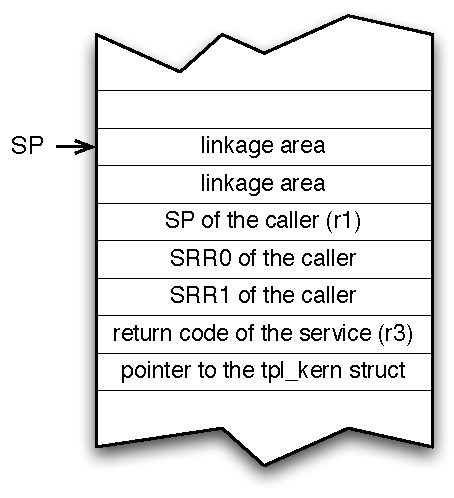
\includegraphics[scale=.6]{pictures/KStackMapping} 
\end{minipage}
\begin{minipage}{0.5\textwidth}
  \caption{Kernel stack mapping after allocation.}\label{fig:kernelstackmapping}
\end{minipage}
\end{figure}

\subsubsection{Calling the service}

Since the registers used to pass parameters to a function, that is \reg{r3} to \reg{r10} as documented in \cite{PPCeabi}, have not been changed until now, calling the function that implements the service respects the register usage conventions.

The first thing to do is to get the function pointer corresponding to the service id. The service id is in \reg{r0} as explained in \ref{sec:systemservices} and is used as an index to the \var{tpl_dispatch_table}.

\begin{lstlisting}[language=C]
  slwi  r0,r0,2                           /* compute the offset    */
  /*
   * load the ptr to the dispatch table
   */
  lis   r11,TPL_HIG(tpl_dispatch_table)     
  ori   r11,r11,TPL_LOW(tpl_dispatch_table)
  lwzx  r11,r11,r0                  /* get the ptr to the service  */
  mtlr  r11                         /* put it in lr for future use */
\end{lstlisting}

The second thing to do is to reset the \var{need_switch} flag that triggers a context switch. This flag (a byte) is located in the \var{tpl_kern} kernel struct. This is done as follow:

\begin{lstlisting}[language=C]
  lis   r11,TPL_HIG(tpl_kern)
  ori   r11,r11,TPL_LOW(tpl_kern)
  stw   r11,KS_KERN_PTR(r1)        /* save the ptr for future use  */
  li    r0,NO_NEED_SWITCH
  stb   r0,20(r11)
\end{lstlisting}

In the future \var{tpl_kern} will be reused, so its address is saved in the kernel stack.

Then, to allow reentrancy for a service call in a hook, the \reg{RI} bit of the \reg{MSR} is set to 1. Without that, a \asfct{sc} cannot be  properly executed.

\begin{lstlisting}[language=C]
  mfmsr r11
  ori   r11,r11,RI_BIT_1
  mtmsr r11
\end{lstlisting}

At last, the service is called:

\begin{lstlisting}[language=C]
  blrl
\end{lstlisting}

\subsubsection{Context switch}

The \var{need_switch} flag that as been possibly modified by the service is now checked to do a context switch if needed.

\begin{lstlisting}[language=C]
  lwz   r11,KS_KERN_PTR(r1) /* get back the tpl_kern address */
  lbz   r12,20(r11)         /* get the need_switch flag      */
  andi. r0,r12,NEED_SWITCH  /* check if a switch is needed   */
  beq   no_context_switch
\end{lstlisting}

A context switch is performed in 3 steps. The first one is the context save of the process that loses the CPU. This step is optional because if the service was a \api{TerminateTask} or a \api{ChainTask}, the context needs not to be saved. This information is in the \var{need_switch} flag. Before doing the actual context save, the return value of the service must be saved in the proper location of the kernel stack. The \cfunction{tpl_save_context} function will read it from this location and expects a pointer to the context saving area or the process in \reg{r3}. \var{s_old}, the address of the context saving area, is in another member of \var{tpl_kern}. At the end, the \var{tpl_kern} address is reread because \reg{r11} has been destroyed in \cfunction{tpl_save_context}. 

\begin{lstlisting}[language=C]
  stw   r3,KS_RETURN_CODE(r1) /* save the return value             */
  andi. r0,r12,NEED_SAVE      /* r12 contains need_switch          */
  beq   no_save
  lwz   r3,0(r11)             /* r11 contains the tpl_kern address */
  bl    tpl_save_context      /* and s_old is put into r3          */
  lwz   r11,KS_KERN_PTR(r1)   /* get back tpl_kern address         */
\end{lstlisting}

The second step consists in loading the configuration of memory protection for the process that get the CPU by calling the \cfunction{tpl_set_process_mp} function. This function expects the id of the process in \reg{r3}. Again this id is located in member \var{proc_id} of \var{tpl_kern}. This is done only if \cmacro{WITH_MEMORY_PROTECTION} is \YES. 

\begin{lstlisting}[language=C]
#if WITH_MEMORY_PROTECTION == YES
  lwz   r3,16(r11) /* get the id of the process which get the cpu  */
  bl    tpl_set_process_mp     /* set the memory protection scheme */
#endif
\end{lstlisting}

The third step loads the context of the process that get the CPU. The address of \var{tpl_kern} is loaded into \reg{r11} because it has been destroyed in \cfunction{tpl_set_process_mp}, \var{s_running}, the address of the context saving area of the current process is loaded into \reg{r3} and \cfunction{tpl_load_context} is called. At last, \reg{r3} is restored.

\begin{lstlisting}[language=C]
  lwz   r11,KS_KERN_PTR(r1)
  lwz   r3,4(r11)                    /* get s_running              */
  bl    tpl_load_context
  lwz   r3,KS_RETURN_CODE(r1)
\end{lstlisting}

\subsubsection{Switching back to the process stack}

At this stage, the \reg{SRR0} and \reg{SRR1} registers saved in the kernel stack are restored. The space reserved in the kernel stack is freed. The reentrancy counter is decremented and the stack switches to the process stack if the reentrancy counter is 0.

\begin{lstlisting}[language=C]
  lwz   r11,KS_SRR0(r1)
  mtspr spr_SRR0,r11
  lwz   r11,KS_SRR1(r1)
  mtspr spr_SRR1,r11

  addi  r1,r1,KS_FOOTPRINT       /*  free back space on the stack  */
  
  /*
   * The reentrency counter is decremented. If it reaches
   * 0, the process stack is restored
   */
  lis   r11,TPL_HIG(tpl_reentrancy_counter)
  ori   r11,r11,TPL_LOW(tpl_reentrancy_counter)
  lwz   r12,0(r11)    /*  get the value of the counter */
  subi  r12,r12,1
  stw   r12,0(r11)
  cmpwi r12,0
  bne   no_stack_restore

  /* 
   * Restore the execution context of the caller
   * (or the context of the task/isr which just got the CPU)
   */
  lwz   r1,KS_SP-KS_FOOTPRINT(r1)   /*  Restore the SP and switch
                                        back to the process stack  */
\end{lstlisting}

\subsubsection{Enabling memory protection}

Then, if memory protection is used, the user scheme is reenabled. The actual works depends on the kind of MPU and is done in \cfunction{tpl_user_mp}.

\begin{lstlisting}[language=C]
#if WITH_MEMORY_PROTECTION == YES
  subi  r1,r1,4
  mflr  r11
  stw   r11,0(r1)   /* save lr on the current stack  */
  bl    tpl_user_mp /* Enable the memory protection  */
  lwz   r11,0(r1)   /* restore lr                    */
  mtlr  r11
  addi  r1,r1,4
#endif
\end{lstlisting}

\subsubsection{Restoring registers}

Registers saved at stage 1 on the process stack are restored an the stack is freed.

\begin{lstlisting}[language=C]
  lwz   r11,PS_CR(r1)
  mtcr  r11
  lwz   r11,PS_LR(r1)
  mtlr  r11
  lwz   r12,PS_R12(r1)
  lwz   r11,PS_R11(r1)

  addi  r1,r1,PS_FOOTPRINT
\end{lstlisting}

\subsubsection{Getting back to the process}

At last, the dispatch layer is exited using a \asfct{rfi}.

\begin{lstlisting}[language=C]
  rfi                                 /* return from interrupt */
\end{lstlisting}

\subsection{Interrupt handler}

\subsection{The CallTrustedFunction service}

The \api{CallTrustedFunction} service is implemented by the \cfunction{tpl_call_trusted_function_service} function. This function is a special case of service because the kernel stack and the process stack have to be modified. In addition, an \api{ExitTrustedFunction} service is implemented to restore the process stack when the trusted function exits. Both services have to be written in assembly language since C does not allow to explicitely modify the stack.

\cfunction{tpl_call_trusted_function_service} performs the following steps:

\begin{penum}
\item check the trusted function id is within the allowed range
\item increment the trusted counter of the calling process
\item build a frame on the process stack to store the registers pushed by a service call except for \reg{r0} and for \reg{SRR0} and \reg{SRR1}; put the address of \api{ExitTrustedFunction} in the \reg{lr} location in the process stack; save \reg{SRR0} and \reg{SRR1} in the process stack
\item get the trusted function address and put it in \reg{SRR0}
\item go back to the dispatch layer
\end{penum}

\subsubsection{Checking the trusted function id}

The id of the trusted function is checked to avoid to call a function at an arbitrary address.

\begin{lstlisting}[language=C]
mov   r11,r3               /* save r3 in r11 b/c it will be destroyed */
cmpw  r3,TRUSTED_FCT_COUNT /* check the id of the trusted function    */
ori   r3,r0,E_OS_SERVICEID /* E_OS_SERVICEID return code              */
bge   invalid_trusted_fct_id
mov   r3,r11               /* restore r3 if trusted function id ok    */
\end{lstlisting}

\subsubsection{Incrementing the trusted counter}

The trusted counter of the process is incremented each time a trusted function is called. When the trusted counter is $>0$, the process is trusted. In such a case, the dispatch layer does not enable memory protection when scheduling the process so it has an unlimited access to the whole addressing space.

\begin{lstlisting}[language=C]
  lwz   r11,KS_KERN_PTR(r1) /* get the ptr to tpl_kern                  */
  lwz   r11,12(r11)         /* get the ptr to the runnning process desc */
  lwz   r12,4(r11)          /* get trusted_count member                 */
  addi  r12,r12,1           /* increment it                             */
  stw   r12,4(r11)          /* put it back in the process desc          */
\end{lstlisting}

\subsubsection{Building the frame}

The frame is used to store the calling context of the trusted function and is shown in figure \ref{fig:tfstackmapping}. The following code builds this frame:

\begin{lstlisting}[language=C]
  /*
   * First get back the process stack pointer
   */
  lwz   r11,KS_SP(r1)
  /*
   * Make room to prepare the call of the trusted function
   */
  subi  r11,r11,PS_TRUSTED_FOOTPRINT_IN
  /*
   * store ExitTrustedFunction as the return address
   */
  lis   r12,TPL_HIG(ExitTrustedFunction)
  ori   r12,r12,TPL_LOW(ExitTrustedFunction)
  stw   r12,PS_LR(r11)
  /*
   * Update the stack pointer
   */
  stw   r11,KS_SP(r1)
  /*
   * second get back SRR0 and SRR1 and save them to the process stack
   */
  lwz   r12,KS_SRR0(r1)
  stw   r12,PS_SRR0_IN(r11)
  lwz   r12,KS_SRR1_IN(r1)
  stw   r12,PS_SRR1(r11)
\end{lstlisting}

\begin{figure}[htbp] %  figure placement: here, top, bottom, or page
\begin{minipage}{0.65\textwidth}
    \centering
  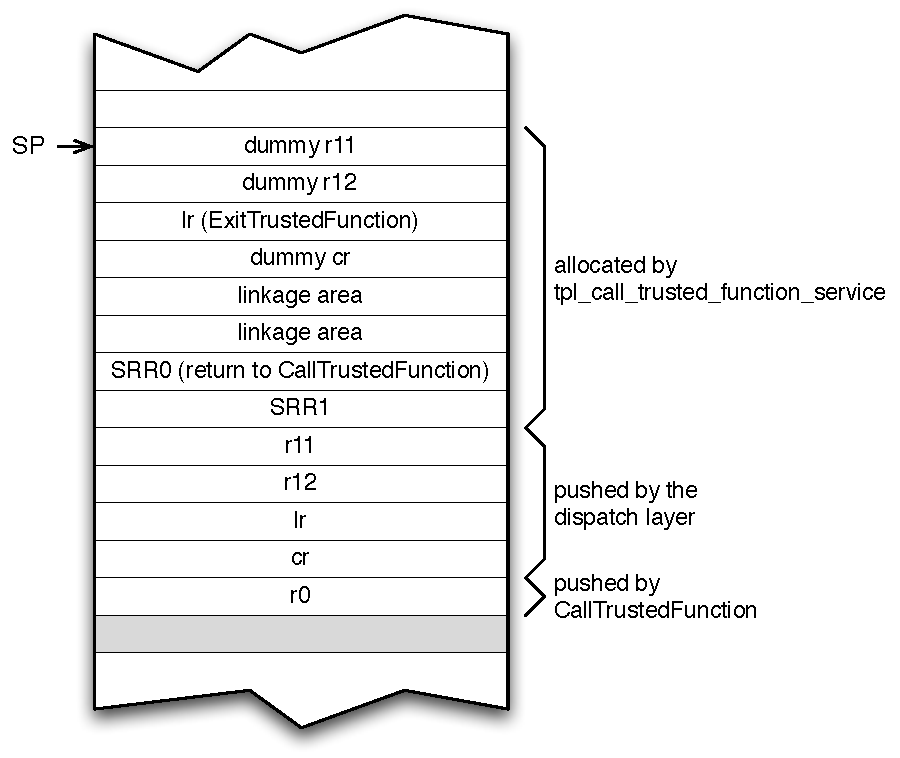
\includegraphics[scale=.6]{pictures/TFStack1} 
\end{minipage}
\begin{minipage}{0.35\textwidth}
  \caption{Process stack mapping at the end of \cfunction{tpl_call_trusted_function_service}. \reg{r0}, at the bottom of the stack has been pushed by \api{CallTrustedFunction}. \reg{cr} to \reg{r11} has been pushed by the dispatch layer. \reg{SRR0} and \reg{SRR1} are saved here by \cfunction{tpl_call_trusted_function_service} to be able to go back to the calling process. Above, the linkage area allows the trusted function to call functions. Above, a frame that will be used by the dispatch layer to restore an execution context for the trusted function is built.}\label{fig:tfstackmapping}
\end{minipage}
\end{figure}

\subsubsection{Setting the trusted function address}

The \reg{SRR0} saved by the dispatch layer after the \api{CallTrustedFunction} is changed to the address of the trusted function. This way, instead of returning to the caller, the trusted function will be executed.

\begin{lstlisting}
  lis   r11,TPL_HIG(tpl_trusted_fct_table)
  ori   r11,r11,TPL_LOW(tpl_trusted_fct_table)
  slwi  r0,r3,2
  lwzx  r12,r11,r0
  stw   r12,KS_SRR0(r1)
\end{lstlisting}

\subsubsection{Going back to the dispatch layer}

A simple \asfct{blr} goes back to the dispatch layer. The latter cleans up the process stack. Once the trusted function starts execution, the process stack is like that:

\begin{figure}[htbp] %  figure placement: here, top, bottom, or page
\begin{minipage}{0.5\textwidth}
    \centering
  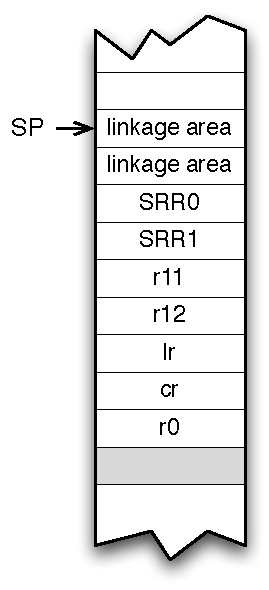
\includegraphics[scale=.6]{pictures/TFStack2} 
\end{minipage}
\begin{minipage}{0.5\textwidth}
  \caption{Process stack mapping when the trusted function starts its execution.}\label{fig:tfstackmapping2}
\end{minipage}
\end{figure}

\subsection{The ExitTrustedFunction service}\label{sec:exittfppc}

When a trusted function finishes, the context of the \api{CallTrustedFunction} must be restored to return to the caller. \api{ExitTrustedFunction} does not need to be called explicitly because its address has been set as the return address of the trusted function by \cfunction{tpl_call_trusted_function_service}. Calling \api{ExitTrustedFunction} explicitly may result in an undefined behavior or in the crash of the calling process but see below. The mapping of the process stack at start of \cfunction{tpl_exit_trusted_function_service} is shown in figure \ref{fig:ETFstack1}.

\begin{figure}[htbp] %  figure placement: here, top, bottom, or page
\begin{minipage}{0.4\textwidth}
    \centering
  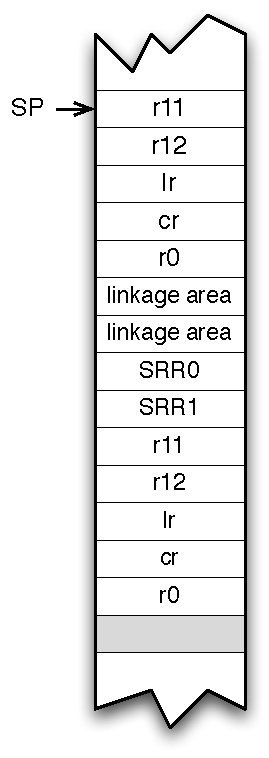
\includegraphics[scale=.6]{pictures/ETFStack1} 
\end{minipage}
\begin{minipage}{0.6\textwidth}
  \caption{Process stack mapping when the \cfunction{tpl_exit_trusted_function_service} function starts its execution.}\label{fig:ETFstack1}
\end{minipage}
\end{figure}

First, \cfunction{tpl_exit_trusted_function_service} decrements the trusted counter of the calling process. A particular attention must be given to this point because by building a fake stack frame and calling Explicitly \api{ExitTrustedFunction} to underflow this counter, a process could get a full access to the memory. So the counter is tested before to avoid to go under 0.

\begin{lstlisting}[language=C]
  lwz   r11,KS_KERN_PTR(r1) /* get the ptr to tpl_kern */
  lwz   r11,12(r11)         /* get the ptr to the runnning process desc */
  lwz   r12,4(r11)          /* get trusted_count member */
  /*
   * Warning, the trusted counter has to be check (compared to 0) to
   * avoid to decrement it if it is already 0. Without that a process
   * could build an had-hoc stack an call explicitly ExitTrustedFunction
   * to get access to all the memory.
   */
  cmpwi r12,0               /* check it is not already at 0 */
  beq   cracker_in_action   /* uh uh */
  subi  r12,r12,1           /* decrement it */
  stw   r12,4(r11)          /* put it back in the process desc */
\end{lstlisting}

\cfunction{tpl_exit_trusted_function_service} has to remove from the process stack the frame that was built by \cfunction{tpl_call_trusted_function_service}, restore \reg{SRR0} and \reg{SRR1} before returning to the dispatch layer.

\begin{lstlisting}[language=C]
cracker_in_action:
  
  /*
   * get the process stack pointer
   */
  lwz   r11,KS_SP(r1)
  
  /*
   * get back the SRR0 and SRR1
   */
  lwz   r12,PS_SRR0_OUT(r11)
  stw   r12,KS_SRR0(r1)
  lwz   r12,PS_SRR1_OUT(r11)
  stw   r12,KS_SRR1(r1)
  
  /*
   * free the process stack and update it in the kernel stack
   */
  addi  r11,r11,PS_TRUSTED_FOOTPRINT_OUT
  stw   r11,KS_SP(r1)
  
  /*
   * that's all
   */
  blr
\end{lstlisting}

\subsection{Execution of the OS Applications startup and shutdown hooks}

These hooks are executed from the kernel but with the access right of a task belonging to the OS Application. The \sysgen\ should choose one of the tasks of the OS Application to be used as context to execute the OS Application startup and shutdown hooks. Execution of an OS Application startup hook is done by the \cfunction{tpl_call_startup_hook_and_resume} function. The argument of this function is a function pointer to the hook. Similarly execution of an OS Application shutdown hook is done by the \cfunction{tpl_call_shutdown_hook_and_resume} function. These functions end by a call to \api{NextStartupHook} and \api{NextShutdownHook} services respectively to cycle through the hooks.

\subsection{The MPC5510 Memory Protection Unit}

The access control rights of the memory region descriptor rules the access of 5 bus masters (labeled from 4 to 0). Unused bus masters are set to the same access right for all the regions. Bus master 4 is used for factory testing only, so the access rights should be set to no access. Bus master 3 is the Flexray controller. Since it is not used in the current version of Trampoline, it is set to no access too. Bus master 2 is the DMA controller and for the same reason it is set to no access. Bus master 1 is the Z0 core. Again it is set to no access.

The access control rights register has the following bit usage:

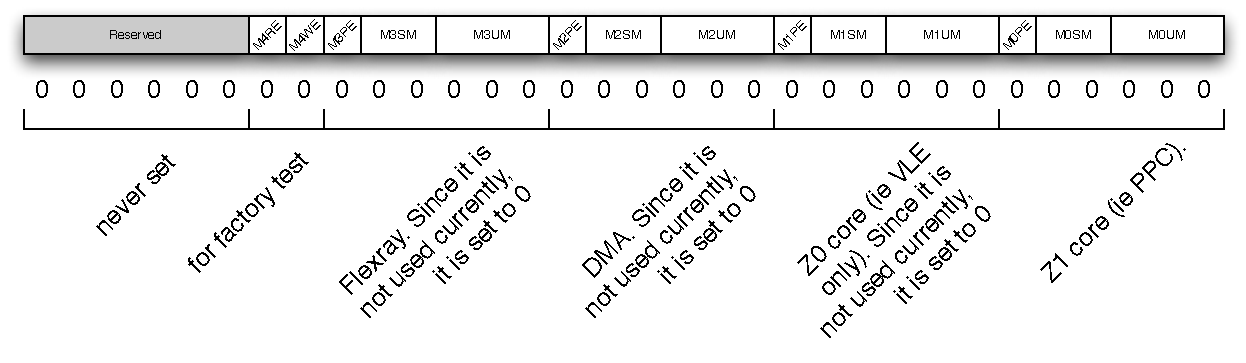
\includegraphics[width=\textwidth]{pictures/MPUacr.pdf} 

Bus master 4 is a special case. The 2 bits have the following meaning:

\rowcolors{1}{white}{light-gray}
\begin{longtable}[c]{l|p{5.15in}}
{\bf Bit}&{\bf Meaning} \\ \hline
\dreg{M4RE} & If set to 1, bus master 4 may {\bf read} memory in the region. If 0, no read is allowed\\
\dreg{M4WE} & If set to 1, bus master 4 may {\bf write} memory in the region. If 0, no write is allowed\
\end{longtable}

So in our case, these bits are set to 0.

Of course, other bus masters have more sophisticated access right:

\rowcolors{1}{white}{light-gray}
\begin{longtable}[c]{l|p{5.15in}}
{\bf Bit}&{\bf Meaning}\\
\hline
\dreg{MxPE} & The PID Enable bit. Set to 0 in our case\\
\dreg{MxSM} & These 2 bits rules the supervisor mode access control with the following meaning: $00=rwx$, $01=rx$, $10=rw$, $11=$ \textit{same as defined by \dreg{MxUM}}. In our case, it is set to $00$ for code and constants and to $11$ for data.\\
\dreg{MxUM} & These 2 bits rules the user mode access control. The first bit means $r$, the second one $w$ and the third one $x$.
\end{longtable}

Trampoline uses 4 descriptors:

\rowcolors{1}{white}{light-gray}
\begin{longtable}{l|p{1.9in}|p{2.6in}}
{\bf Descriptor} & {\bf Usage} & {\bf \dreg{MxUM} value}\\
\hline
\dreg{MPU_RGD0} & Constants and program\footnote{This region is set to the whole addressing space. This is not definitive and should be improved because reading a peripheral control register should be protected. So an additional descriptor has to be used to allow the kernel (supervisor mode) a complete access on all the memory space and no access at all for applications (user mode).}. & $rwx=00$ for supervisor mode, $rx=101$ for user mode.\\
\dreg{MPU_RGD1} & Private variables of the process. & $rw=110$ for supervisor and user mode.\\
\dreg{MPU_RGD2} & Stack of the process. & $rw=110$ for supervisor and user mode.\\
\dreg{MPU_RGD3} & Variables of the OS Application if OS Applications are used. & $rw=110$ for supervisor and user mode.\\
\end{longtable}

So values of access control bits should be:

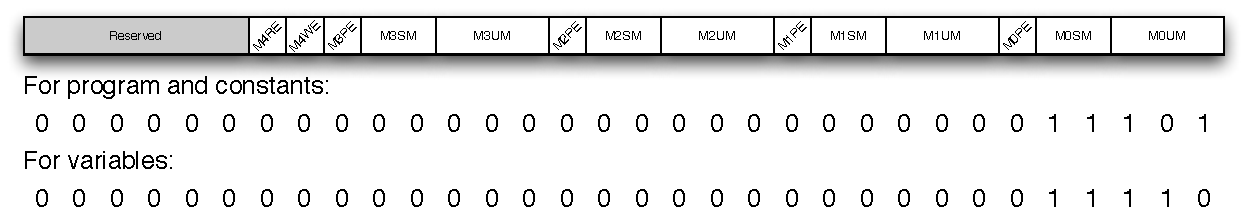
\includegraphics[width=\textwidth]{pictures/MPUprog.pdf} 

So in hexa:

\rowcolors{1}{white}{light-gray}
\begin{longtable}{l|l}
{\bf Kind} & {\bf Value}\\
\hline
Program region access & $0x00000005$\\
Variable region access & $0x0000001E$\\
\end{longtable}

\subsubsection{What happen in case of memory protection violation ?}

Two exception handler are used to handle a memory protection violation, one for data access, one for code access.

The Data Storage exception is tied to the IVOR~2 vector (VPR offset = 0x020), see page 8-2 of the {\em MPC5510 Microcontroller Family Reference Manual}.

The Instruction Storage exception is tied to the IVOR~3 vector (VPR offset = 0x030), see page 8-2 of the {\em MPC5510 Microcontroller Family Reference Manual}.

However, it appears one of these exceptions is raised when the processor is in user mode. The behavior is different in supervisor mode {\em to be completed}.

\section{ARM -- Common conventions}

\subsection{File hierarchy}

\subsection{Common definitions}

\subsection{Bootstraping}

The bootstrap must be made in specific ARM port and must call the \cfunction{main} function. If \cfunction{main} ever returns, the bootstrap code must fall into an infinite loop.

As a reason, many ARM architectures needs early specific and required initializations. This includes steps like memory mapping configuration, DRAM controller configuration, ...

Besides specific initializations, the bootstrap should :
\begin{itemize}
\item initialize stack pointer for every ARM exception modes
\item keep all external interrupts locked (will be unlocked at the first task context loading)
\item call \cfunction{main} in "system" mode (0x1F)
\end{itemize}

\subsection{Stacks}

\subsection{Interrupt management}

Kernel is not interruptible. So hardware interrupt source are disabled entering in kernel (via any case in system call, interrupt request, abort, ...).

But kernel shall be reentrant via system call (because kernel hooks can call some system calls).

\subsubsection{Interrupt and category classification}

All ARM IRQ are category 2 ISR.

All ARM FIQ are category 1 ISR.

\subsubsection{Vector table}

Each ARM exception vector points on a so called "primary" subprogram (like \cfunction{tpl\_primary\_syscall\_handler}).

To be located at address 0x00000000, this vector table is assigned to a specific section named \cfunction{.vectbl}. The linker script uses this section name to output it to address 0x00000000.

\subsubsection{System call}

\subsubsection{IRQ handling}

\subsubsection{FIQ handling}

\section{ARM -- ARM926 chip support}

\label{arm926mmu}

\subsection{Memory protection}

To be written...

Some points to explain :
\begin{itemize}
\item FCSE mechanism is not used by this port (if someone is interested by this work, she's welcome)
\item address translation is not used, all VMA equals physical address
\item IDLE task's memory protection configuration is used to provide configuration for trusted applications or kernel
\end{itemize}

\subsubsection{MMU tables generation principle}

To be written...

Some points to explain :
\begin{itemize}
\item MMU is not disabled in privileged mode, but all useful memory areas are accessible. Thus, we hope we can find bugs easily in privileged code.
\item useful memory areas, except processes and applications ones, are configured as accessible (read and write) in privileged mode. These memory areas are called system areas
\item some memory areas needs to be accessible by anyone (API, GCC builtin functions, common libraries, ...), they are called common areas (they are read only for unprivileged contexts)
\item there is one translation table for each process
\item all translation tables have the same system and common areas
\item there is one page table set for each process. Page tables are fine page tables. Table entries are tiny page descriptors.
\item the number of page table in a set depends on the size of the whole trampoline and application memory footprint. Then this information is given by linker via a symbol which is used by the MMU driver.
\item Page tables are accessed via a macro, as they are allocated by linker (and we cannot know the number of page tables)
\end{itemize}

\subsection{CPU cache support}

\section{ARM -- Armadeus APF27 board}

\subsection{Debugging with Abatron BDI2000 or BDI3000 JTAG probe}

A configuration file is provided in \file{machines/arm/arm926/armadeus-apf27/bdi-config}.

To enable JTAG, if your APF27 has a FPGA, you must load the FPGA to wake it up (TO DO : explain how to do this...).

To start a debug session, follow these steps :
\begin{enumerate}
\item connects everything together
\item power up everything
\item reset the APF27 (S2 on APF27-Dev)
\item stop u-boot before it loads Linux (if MMU is started, you won't be able to load anything)
\item telnet your BDI
\item type \cfunction{reset} command in the BDI shell
\item start GDB session (\cfunction{target remote ...})
\end{enumerate}

\subsection{Configuration}

All configuration of port is done in \file{apf27\_config.h}.

\subsubsection{Stacks}

Stacks' size (stack of each exception mode) can be adjusted via the following constants. Remember that the size must be aligned to 4.

\subsubsection{CPU caches}

By default, CPU caches are disabled (for real time determinism).

\subsection{Memory mapping}

This port can be use in one of these three configurations :
\begin{enumerate}
\item No memory mapping (and thus no memory protection)
\item Memory mapping without memory protection
\item Memory mapping and memory protection
\end{enumerate}

\subsection{Memory protection}

Memory protection is based on ARM926 shared code (see~\ref{arm926} page~\pageref{arm926})

\section{ARM -- Simtec EB675001 board}

\subsection{Memory map and hardware resources}

Talk about configured memory map (use of DRAM, where the bootstrap would be flashed, \ldots).

Tell which hardware resources are used by the kernel.

\subsection{Booting}

There is two way to start Trampoline on APF27 :
\begin{itemize}
\item from ELF image (in file usually called \file{trampoline})
\item from raw binary image (in file usually called \file{trampoline.bin})
\end{itemize}

\subsubsection{Booting from ELF image}

Load image with your ELF loader (the file is usually named \file{trampoline}). This can be GDB via a JTAG probe for example. Then, just start execution from \cfunction{tpl\_arm\_bootstrap\_entry} entry point. Here are commands you can type in GDB :
\begin{lstlisting}
(gdb) load
(gdb) set $pc=tpl_arm_bootstrap_entry
(gdb) break main
(gdb) continue
\end{lstlisting}

\subsubsection{Booting from raw binary image}

Load image with your binary loader to 0xA0000000 memory address. Then just start execution at this point (0xA0000000).

With u-boot, you can type these commands :
\begin{lstlisting}
BIOS> tftpboot 0xA0000000 192.168.5.20:trampoline.bin
BIOS> go 0xA0000000
\end{lstlisting}

\subsection{Internal kernel drivers}

\subsection{Hardware interrupts handling}

\subsection{Idle task}

\subsection{Exceptions handling}

\subsection{Kernel sleep service}


\section{ARM - Cortex}

\subsection{Overview}

\subsubsection{The processor}

The processor has two modes of execution depending on the kind of execution.
The processor modes are:
\begin{penum}
\item Thread mode: Used to execute application software.
The processor enters Thread mode when it comes out of reset.
The CONTROL register controls whether software execution is privileged or unprivileged, see CONTROL register on page 24.
\item Handler mode: Used to handle exceptions.
The processor returns to Thread mode when it has finished exception processing.
Software execution is always privileged.
\end{penum}

The privilege levels for software execution are:
\begin{penum}
\item Unprivileged: Unprivileged software executes at the unprivileged level and:
	\begin{penum}
	\item Has limited access to the MSR and MRS instructions, and cannot use the CPS instruction
	\item Cannot access the system timer, NVIC, or system control block
	\item Might have restricted access to memory or peripherals
	\item Must use the SVC instruction to make a supervisor call to transfer control to privileged software
	\end{penum}
\item Privileged: Privileged software executes at the privileged level and can use all the instructions and has access to all resources.
Can write to the CONTROL (nPRIV : bit 0) register to change the privilege level for software execution.
\end{penum}

Core processor registers are depicted in figure \ref{fig:CM4core}.

\begin{figure}[htbp] %  figure placement: here, top, bottom, or page
\begin{minipage}{0.5\textwidth}
    \centering
  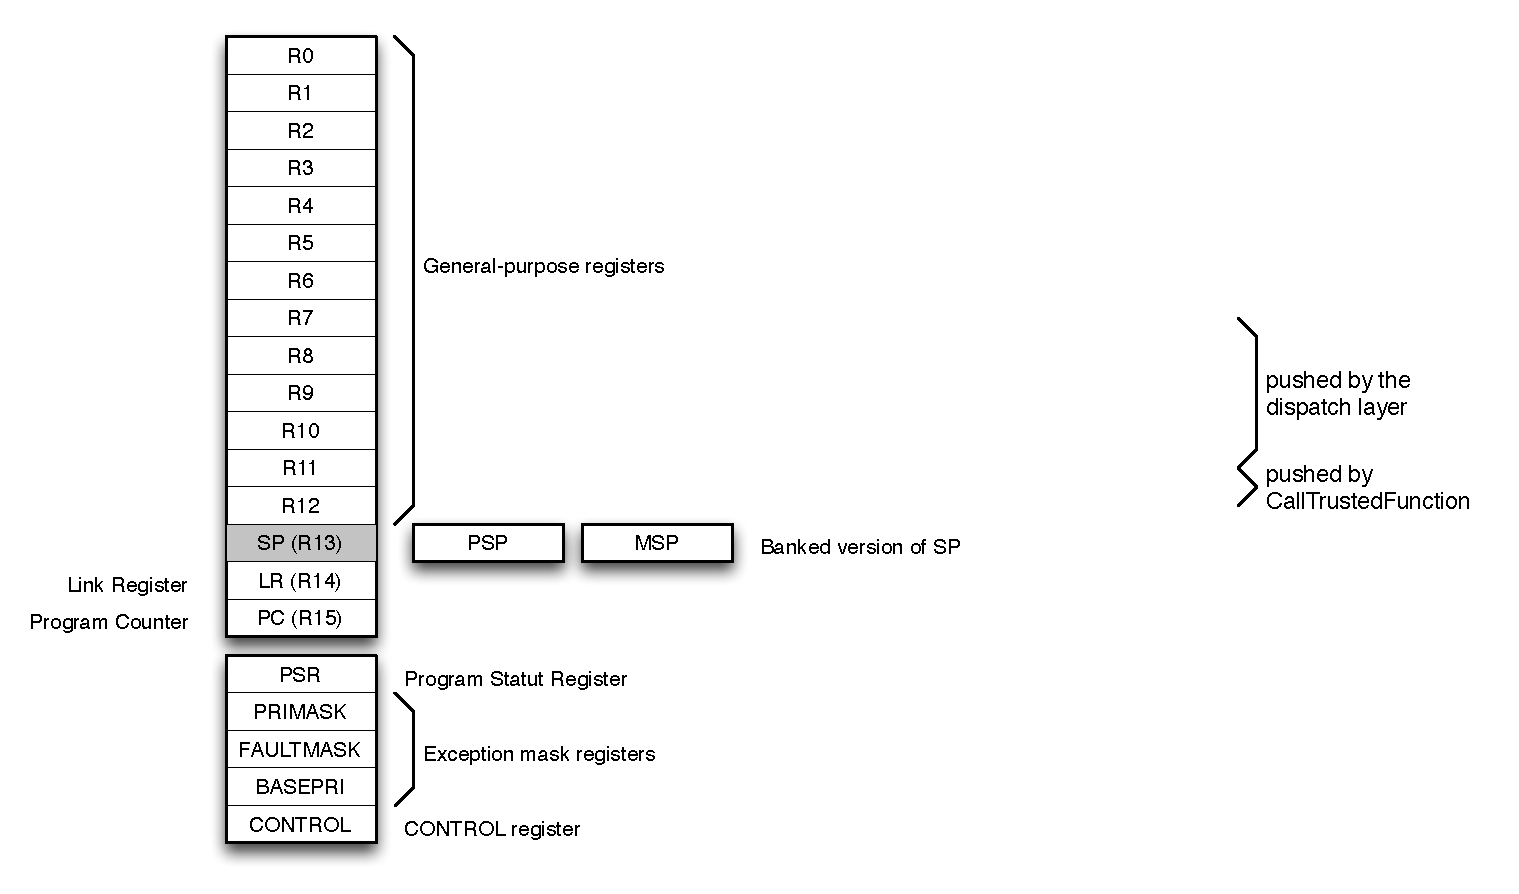
\includegraphics[scale=.6]{pictures/CM4core} 
\end{minipage}
\begin{minipage}{0.5\textwidth}
   \caption{Processor core registers}\label{fig:CM4core}
\end{minipage}
\end{figure}

The Program Status Register (PSR) combines:
\begin{penum}
\item Application Program Status Register (APSR)
\item Interrupt Program Status Register (IPSR)
\item Execution Program Status Register (EPSR)
\end{penum}

These registers are mutually exclusive bitfields in the 32-bit PSR.

\subsubsection{The stack}
The processor uses a full descending stack. This means the stack pointer indicates the last stacked item on the stack memory. When the processor pushes a new item onto the stack, it decrements the stack pointer and then writes the item to the new memory location. The processor implements two stacks, the main stack and the process stack, with independent copies of the stack pointer.
In Thread mode, the \reg{CONTROL} register controls whether the processor uses the main stack or the process stack. In Handler mode, the processor always uses the main stack.
The options for processor operations are:

\begin{longtable}[c]{llllp{3cm}}
\toprule
{\bf Processor mode} & {\bf Used to execute} & {\bf Privilege level for execution} & {\bf Stack used} \\
\midrule
Thread & Applications & Privileged or unprivileged & Main stack or Process stack \\
Handler & Exception handlers & Always privileged & Main stack \\
\bottomrule
\end{longtable}

The port of Trampoline will use the two stacks and unprivileged level for software execution. This configuration is made in the function \cfunction{tpl_init_machine_generic} of file \file{tpl_machine_arm_generic.c}:

\begin{lstlisting}[language=C]
FUNC (void, OS_CODE) tpl_init_machine_specific (void)
{
  tpl_kernel_stack_top = (uint32)&tpl_kernel_stack[KERNEL_STACK_SIZE - 1];
  nested_kernel_entrance_counter = 0;
  __set_MSP(tpl_kernel_stack_top); 
  setTimer();
  __set_CONTROL(0x3); /* Switch to use Process Stack, privileged state */
  __ISB(); /* Execute ISB after changing CONTROL register */
}
\end{lstlisting}

On reset the processor starts in Thread mode and uses the Main stack (\reg{MSP}) for both Handler and Thread modes.
We set the Process stack to the current Main stack address and switch to use Process stack for Thread mode.
We then set the Main stack to a dedicated area pointed to by ptrMainStack.

\subsubsection{The memory}

The processor has a fixed memory map that provides up to 4 GB of addressable memory.

\subsubsection{The exceptions}

The Cortex-M4 processor supports interrupts and system exceptions. The processor and the Nested Vectored Interrupt Controller (NVIC) prioritize and handle all exceptions. The processor uses handler mode to handle all exceptions except for reset.
The NVIC registers control interrupt handling and includes the following features:
\begin{penum}
\item 82 maskable interrupt channels for STM32F407xx (not including the 16 interrupt lines of CortexTM-M4 with FPU)
\item 16 programmable priority levels (4 bits of interrupt priority are used)
All interrupts including the core exceptions are managed by the NVIC
\end{penum}

\begin{longtable}[c]{llllp{5cm}}
\toprule
{\bf Exception number} & {\bf Priority} & {\bf Type} & {\bf Priority} \\
\midrule
1 & & Reset & -3 the highest \\
\hline
2 & -14 & NMI & -2 \\
\hline
3 & -13 & Hard fault & -1 \\
\hline
4 & -12 & Memory management fault & Configurable \\
\hline
5 & -11 & Bus fault & Configurable \\
\hline
6 & -10 & Usage fault & Configurable \\
\hline
7-10 & & & \\
\hline
11 & -5 & SVCall & Configurable \\
\hline
12-13 & & & \\
\hline
14 & -2 & PendSV & Configurable \\
\hline
15 & -1 & SysTick & Configurable \\
\hline
16-above & 0 and above & Interrupt (IRQ) & Configurable \\
\bottomrule
\end{longtable}

When an exception arises the processor saves a context state onto a stack pointed to by \reg{sp} (either \reg{MSP} or \reg{PSP} depending on the mode of the processor at the time of the exception) and jumps to the Supervisor Call handler. The context state supports the \textit{ARM Architecture Procedure Calling Standard} (AAPCS).
When pushing context to the stack, the hardware saves eight 32-bit words, comprising xPSR, ReturnAddress, LR (R14), R12, R3, R2, R1, and R0. This behaviour is depicted figure \ref{fig:CM4StackExceptionEntry}.

\begin{figure}[htbp] %  figure placement: here, top, bottom, or page
\begin{minipage}{0.5\textwidth}
    \centering
  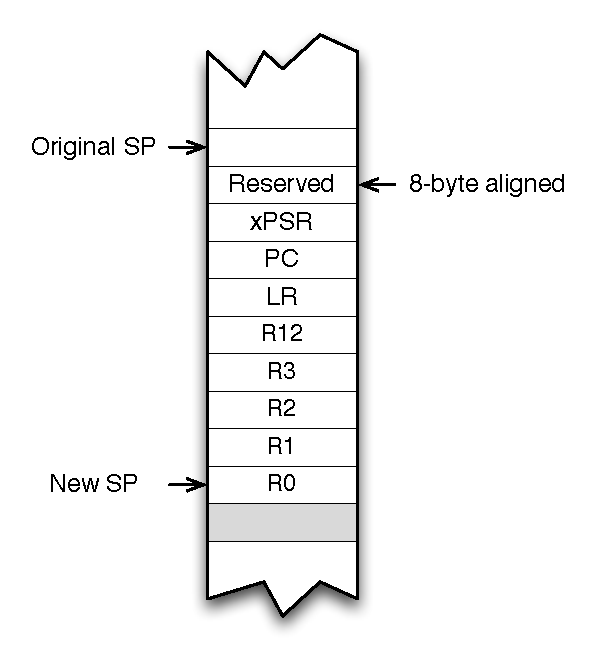
\includegraphics[scale=.6]{pictures/CM4StackExceptionEntry} 
\end{minipage}
\begin{minipage}{0.5\textwidth}
   \caption{Stacking frame upon exception rising}\label{fig:CM4StackExceptionEntry}
\end{minipage}
\end{figure}

\subsection{System services} \label{sec:systemservices}

The Cortex-M4 port uses the \asfct{svc} (Supervisor Call) exception call to call system services \cite{}.

The id of the system service to call is given in the \reg{r0} register and \reg{r0} save and restore are added around.
A system service may be directly called (without using the Supervisor Call) in case of nested calls. This is due to the architecture of the Cortex-m4. Other microcontrolers (e.g. Power PC) have features that enable nested system calls.

For instance, the following listing gives the \api{ActivateTask} service code. These functions are generated from templates by goil (see \ref{sec:generatedfiles}) and are part of the {\em invoque} layer (see \ref{sec:invoque}):

\begin{lstlisting}[language=C]
	/* 
	 * Service ActivateTask
	 */
	.global ActivateTask
	.type   ActivateTask, %function
ActivateTask:
	/* manage reentrance of kernel */
	ldr r1, =nested_kernel_entrance_counter
	ldr r2, [r1]
	/* If nested_kernel_entrance_counter is greater or equal than 1 */
	cmp r2,#1
	/* then we are in Handler mode and we must call the service with a 
	 * direct call to the function */
	beq ActivateTask_direct_call
	/* Exception call to the service : use SVC exception */
ActivateTask_exception_call:
	mov r3,#OSServiceId_ActivateTask
	svc #OSServiceId_ActivateTask
	b ActivateTask_exit_call
	/* Procedural call to the service */
ActivateTask_direct_call:
	/* get the appropriate system call address into R3 */
	ldr r1, =tpl_dispatch_table
	mov r3, #OSServiceId_ActivateTask
	ldr r3, [r1, r3, LSL #2]
	push {lr}
	/* call the service  */
	blx r3
	pop {lr}
	/* Function call */
ActivateTask_exit_call:
	bx lr
\end{lstlisting}

The \textit{ARM Architecture Procedure Calling Standard} (AAPCS) defines the following behaviour for subroutine call:
\begin{longtable}[c]{l l l p{5cm}}
\toprule
{\bf Register} & {\bf Synonym} & {\bf Special} & {\bf Role in the procedure call standard} \\
\midrule
r15 & & PC & -3 The Program Counter \\
\hline
r14 & & LR & The Link Register \\
\hline
r13 & & SP & The Stack Pointer \\
\hline
r12 & & IP & The Intra-Procedure-call Scratch-register \\
\hline
r11 & v8 & & Variable-register 8 \\
\hline
r10 & v7 & & Variable-register 7 \\
\hline
r9 & & v6, SB, TR & Platform register. The meaning of this register is defined by the platform standard. \\
\hline
r8 & v5 & SVCall & Variable-register 5 \\
\hline
r7 & v4 & & Variable-register 4 \\
\hline
r6 & v3 & PendSV & Variable-register 3 \\
\hline
r5 & v2 & SysTick & Variable-register 2 \\
\hline
r4 & v1 & & Variable-register 1 \\
\hline
r3 & a4 & & Argument / Scratch-register 4 \\
\hline
r2 & a3 & & Argument / Scratch-register 3 \\
\hline
r1 & a2 & & Argument / Scratch-register 2 \\
\hline
r0 & a1 & & Argument / Scratch-register 1 \\
\bottomrule
\end{longtable}

Where the role of registers are:
\begin{penum}
\item \textbf{Scratch-register}, \textbf{Temporary-register} : A register used to hold an intermediate value during a calculation (usually, such values are not named in the program source and have a limited lifetime).
\item \textbf{Variable-register}, \textbf{V-register} : A register used to hold the value of a variable, usually one local to a routine, and often named in the source code.
\end{penum}

\subsection{Dispatching the service call}

Raising the \asfct{svc} exception makes the processor change the stack pointer from the Process Stack Pointer to the Main Stack Pointer and then save a set of registers on top of this Main Stack.
The kernel stack is the Main Stack and the process stack is the Process Stack.

The Cortex-M4 locates the Supervisor Call handler in the exception handler 11. 
but, depending on the CPU kind, it may be located elsewhere. Since the available memory for the interrupt or exception handler may vary, a jump is made to the \cfunction{tpl_primary_syscall_handler}.%:

\cfunction{tpl_primary_syscall_handler} performs the following tasks:
\begin{penum}
\item Prepare the environment
\item Saves additional registers to be able to work
\item Disables memory protection
\item Switches to kernel stack if needed
\item Calls the service
\item Performs a context switch if needed and programs the MPU.
\item Switches back to the process stack if needed
\item Enable memory protection
\item Restore registers
\item Get back to the process
\end{penum}

\note{Currently the Cortex-M4 port does not support tasks that use floating point registers}

\subsubsection{Preparing the environment}

When the Supervisor Call begins execution, the process stack has the mapping depicted in figure \ref{fig:CM4StackAfterInvoque}.

\begin{figure}[htbp] %  figure placement: here, top, bottom, or page
\begin{minipage}{0.5\textwidth}
    \centering
  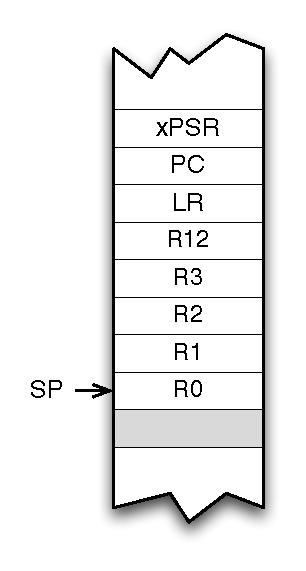
\includegraphics[scale=.6]{pictures/CM4StackAfterInvoque} 
\end{minipage}
\begin{minipage}{0.5\textwidth}
   \caption{Process stack mapping at the beginning of the Supervisor Call handler. The grayed zone represents an unknown content depending on from where the service was called.}\label{fig:CM4StackAfterInvoque}
\end{minipage}
\end{figure}

We will need space on top of current stack (Main stack or Kernel stack) \reg{MSP} in order to save working registers.
Some registers could be found in the frame saved by the processor, but we kept a common scheme for handling exception calls.

\subsubsection{Saving additional registers}

We save following values and registers on top of kernel stack :
\begin{itemize}
\item The value of caller \reg{sp} : 
\item Register \reg{lr} : This register is modified when calling subroutines. We save it to properly restore the caller process stack.
\item Return code, the return code of service : The return code of the service is stored into \reg{R0} register when returning from service. We save it into kernel stack as soon as the return of the service so that we can transmit it to the caller of service.
\item A pointer to \var{tpl_kern}
\item \reg{r4} : Working register
\item \reg{r5} : Working register
\end{itemize}


Additional values saving is done by the following code at start of the \cfunction{tpl_sc_handler} and the mapping of the kernel stack is depicted at figure \ref{fig:CM4KernelStackSaveDone}:

\begin{lstlisting}[language=C]
  sub sp, sp, #KS_FOOTPRINT /* Make space on top of kernel stack. */
  mrs r12, psp /* Copy process stack pointer psp into r12 */
  str r12, [sp, #KS_PROCESS_SP] /* and save it into kernel stack. */
  str r4, [sp, #KS_R4]	 /* Save working register r4 on process stack. */
  str r5, [sp, #KS_R5] /* Save working register r5 on process stack. */
  ldr r12, =tpl_kern
  str r12, [sp, #KS_KERN_PTR] /* Store tpl_kern into kernel stack. */
  str lr, [sp, #KS_LR] /* Store lr register into kernel stack. */
\end{lstlisting}

\subsubsection{Disabling memory protection}

This part of the dispatch layer is done in the \cfunction{tpl_enter_kernel} function and is assembled only if \cmacro{WITH_MEMORY_PROTECTION} is set to \YES. After pushing the \reg{lr} on the kernel stack, the \cfunction{tpl_kernel_mp} function is called and does the actual job. At last \reg{lr} is popped from the kernel stack.

\begin{lstlisting}[language=C]
#if WITH_MEMORY_PROTECTION == YES
  /*
   * Switch to kernel memory protection scheme
   */
  push {lr}
  bl tpl_kernel_mp
  pop {lr}
#endif
\end{lstlisting}

\subsubsection{Switching to the kernel stack}

The Cortex-m4 is configured to use two stacks and the Main Stack is the kernel stack.

The kernel stack may be already used because a call to a \cfunction{PreTaskHook} or a \cfunction{PostTaskHook} is done on the kernel stack and such a hook may call a service. So the dispatch layer must be reentrant. The number of reentrant calls is counted by the \var{tpl_reentrancy_counter}. For a reentrant call, the same frame is build over the current one.

\begin{lstlisting}[language=C]
  /* 
   * Manage reentrance of kernel
   * Increment nested_kernel_entrance_counter
  */
  ldr r12, =nested_kernel_entrance_counter
  ldr r4, [r12]
  add r4, r4, #1
  str r4, [r12]
\end{lstlisting}

\begin{figure}[htbp] %  figure placement: here, top, bottom, or page
\begin{minipage}{0.5\textwidth}
    \centering
  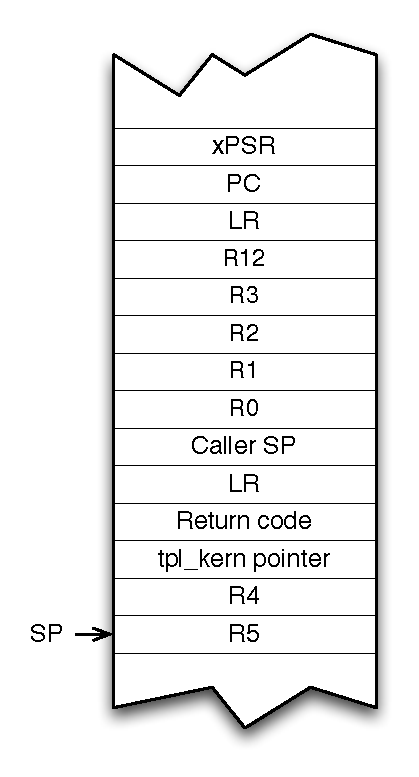
\includegraphics[scale=.6]{pictures/CM4KernelStackSaveDone} 
\end{minipage}
\begin{minipage}{0.5\textwidth}
   \caption{Kernel stack mapping after saving additional registers.}\label{fig:CM4KernelStackSaveDone}
\end{minipage}
\end{figure}

\subsubsection{Calling the service}

Since the registers used to pass parameters to a function, that is \reg{r3} to \reg{r10} as documented in \cite{PCSAA}, have not been changed until now, calling the function that implements the service respects the register usage conventions.

The first thing to do is to get the function pointer corresponding to the service id. The service id is in \reg{r0} as explained in \ref{sec:systemservices} and is used as an index to the \var{tpl_dispatch_table}.

\begin{lstlisting}[language=C]
  /*
   * Get the appropriate system call address into R3
   */
  ldr r12, =tpl_dispatch_table
  ldr r3, [r12, r3, LSL #2]
\end{lstlisting}

The second thing to do is to reset the \var{need_switch} flag that triggers a context switch. This flag (a byte) is located in the \var{tpl_kern} kernel struct. This is done as follow:

\begin{lstlisting}[language=C]
  /*
   * Reset tpl_kern variables
   */
  ldr r12, [r5, #KS_KERN_PTR] /* load the tpl_kern base address from kernel stack */
  mov r4, #NO_NEED_SWITCH_NOR_SCHEDULE
  strb r4, [r12, #TPL_KERN_OFFSET_NEED_SWITCH]
  strb r4, [r12, #TPL_KERN_OFFSET_NEED_SCHEDULE]
\end{lstlisting}

At last, the service is called:

\begin{lstlisting}[language=C]
  blx r3
\end{lstlisting}

And we then immediately save the return value of the service call into the kernel stack:
\begin{lstlisting}[language=C]
  str r0, [r5, #KS_RETURN_CODE]
\end{lstlisting}

\subsubsection{Context switch}

The \var{need_switch} flag that as been possibly modified by the service is now checked to do a context switch if needed.

\begin{lstlisting}[language=C]
  ldr r12, [r5, #KS_KERN_PTR] /* load the tpl_kern base address */
  ldrb r12, [r12, #TPL_KERN_OFFSET_NEED_SWITCH]
  cmp r12, #NO_NEED_SWITCH
  beq no_context_switch
\end{lstlisting}

A context switch is performed in 3 steps:
\begin{itemize}
\item Save the context of the task that looses the cpu.
\item Load the configuration of memory protection for the process that gets the cpu.
\item Load the context of the process that get the cpu.
\end{itemize}

\paragraph{Save the context of the task th	at looses the cpu}

The first one is the context save of the process that loses the CPU. This step is optional because if the service was a \api{TerminateTask} or a \api{ChainTask}, the context needs not to be saved. This information is in the \var{need_switch} flag. \var{s_old}, the address of the context saving area, is in another member of \var{tpl_kern}. 

\begin{lstlisting}[language=C]
  ldr r12, [r5, #KS_KERN_PTR] /* load the tpl_kern base address */
  ldr r12, [r12, #TPL_KERN_OFFSET_S_RUNNING]
  push {lr}
  bl tpl_save_context
  pop {lr}
\end{lstlisting}

\paragraph{Load the configuration of memory protection for the process that gets the cpu}

TODO
(
The second step consists in loading the configuration of memory protection for the process that get the CPU by calling the \cfunction{tpl_set_process_mp} function. This function expects the id of the process in \reg{r3}. Again this id is located in member \var{proc_id} of \var{tpl_kern}. This is done only if \cmacro{WITH_MEMORY_PROTECTION} is \YES. 

\begin{lstlisting}[language=C]
#if WITH_MEMORY_PROTECTION == YES
  lwz   r3,16(r11) /* get the id of the process which get the cpu  */
  bl    tpl_set_process_mp     /* set the memory protection scheme */
#endif
\end{lstlisting}
)

\paragraph{Load the context of the process that get the cpu}

The third step calls the function \cfunction{tpl_run_elected}. This function chooses the process that will get the cpu and write this information into the field \var{tpl_kern.s_running}.

Then we load the context of the process that got the CPU. The address of \var{tpl_kern} is loaded into \reg{r12} because it has been destroyed in \cfunction{tpl_set_process_mp}, \var{s_running}, the address of the context saving area of the current process is loaded into \reg{r12} and \cfunction{tpl_load_context} is called.

\begin{lstlisting}[language=C]
  ldr r12, [r5, #KS_KERN_PTR]	/* load the tpl_kern base address */
  ldr r12, [r12, #TPL_KERN_OFFSET_S_RUNNING] /* get the address of the context bloc */
  push {lr}
  bl tpl_load_context
  pop {lr}
\end{lstlisting}

\subsubsection{Switching back to the process stack}

This is not useful for the Cortex-m4.

\subsubsection{Leaving the kernel}

Now we leave the kernel by calling the subroutine \cfunction{tpl_leave_kernel}
\begin{lstlisting}[language=C]
  push {lr}
  bl tpl_leave_kernel
  pop {lr}
\end{lstlisting}

In this routine the reentrancy counter is decremented by 1.

\subsubsection{Enabling memory protection}

Then, if memory protection is used, the user scheme is reenabled. The actual works depends on the kind of MPU and is done in \cfunction{tpl_user_mp}.

\begin{lstlisting}[language=C]
#if WITH_MEMORY_PROTECTION == YES
  /*
  * Switch to user memory protection scheme
  */
  push {lr}
  bl tpl_user_mp
  pop {lr}
#endif
\end{lstlisting}

\subsubsection{Restoring registers}

Registers saved at stage 1 on the kernel stack are restored and the stack is freed.

\begin{lstlisting}[language=C]
  ldr r4, [sp, #KS_R4]
  ldr r5, [sp, #KS_R5]
  ldr lr, [sp, #KS_LR]

  ldr r12, [sp, #KS_PROCESS_SP]
  msr psp, r12
  add sp, sp, #KS_FOOTPRINT	
\end{lstlisting}

\subsubsection{Getting back to the process}

At last, the dispatch layer is exited using a \asfct{bx}.

\begin{lstlisting}[language=C]
tpl_sc_handler_exit:
  bx lr
\end{lstlisting}

\subsection{Cortex-M FPU support}

Processors with a floating-point unit add the following registers to the context:
\begin{itemize}
\item 32 32-bits registers named \reg{s0} to \reg{s31} which can be seen as 16 64-bit registers named \reg{d0} to \reg{d15} for instructions operating on double-precision floating-point numbers.
\item \reg{fpscr} is the floating-point status and control register.
\end{itemize}

\reg{fpsid} is the floating-point system ID register but as this register seems to be read-only, it is not part of the context.

From the ARMv7-M Architecture Reference Manual (\texttt{DDI 0403E.e}), 3 different context state stacking methods are available on exception entry with the FP extension (section \texttt{B 1.5.7}):
\begin{itemize}
  \item do not stack any FP context (by hardware)
  \item stack an extended frame context, including the integer basic frame and volatile FP registers (\texttt{s0} to \texttt{s15} and \texttt{fpscr})
  \item an intermediate approach, named \textsl{lazy context save}, that reserves place on the stack, but writes data only if needed, \textsl{i.e.} if there is an FPU related instruction during the exception. This is the default behavior.
\end{itemize}

In Trampoline, we choose to deal with the FP context in software only, as:
\begin{itemize}
  \item we need to use both FPU enabled tasks and integer only tasks, and the context does not always need to be saved (end of a job with \texttt{TerminateTask} for instance). 
  \item The last 2 approaches are interesting because they don't require the use of an assembler part, but in our case the interest is limited (we already have assembly…)
\end{itemize}

\subsubsection{Data structure}

When floating point is activated, the static task descriptor has an additional member, a pointer to the floating point context structure, which is located just after the pointer to the integer context structure. Function that save and load the context, \cfunction{tpl_save_context}, \cfunction{tpl_load_context}, \cfunction{tpl_save_context_under_it} and \cfunction{tpl_load_context_under_it} all have a pointer to the static task descriptor in \reg{r0} register. The floating context is accessed by reading its pointer. If the pointer is \constant{NULL}, the is not saved:

\begin{lstlisting}[language=C]
  ldr r1,[r0,#FLOAT_CONTEXT]
  cmp r1,#0
  beq no_save_fp
\end{lstlisting}

Saving the floating-point context needs to save \texttt{spr} registers and the \texttt{fpscr} status register.

\begin{lstlisting}[language=C]
  /* save all s0 to s31 */
  vstm r1!, {s0-s31}
  /* save fpscr */
  vmrs r0,fpscr
  str r0,[r1]
\end{lstlisting}

Loading the floating-point context is the same reversed. Assuming \reg{r1} is loaded with a pointer to the floating-point context. Remember that if the pointer is \constant{NULL}, these instructions are skiped:

\begin{lstlisting}[language=C]
#if WITH_FLOAT == YES
  /*-------------------------------------------------------------------------
   * Get a the pointer to the floating point context from the pointer to the
   * static descriptor of the running task
   */
  ldr r1,[r0,#FLOAT_CONTEXT]
  cmp r1, #0 /* r1 is NULL if there is no float context for this process */
  beq no_load_fp
  vldm r1!, {s0-s31} /* load s[0..31] */
  ldr r0,[r1]
  vmsr fpscr, r0 /* load fpscr */
no_load_fp:
#endif // WITH_FLOAT
\end{lstlisting}

\subsubsection{Lazy Context Switch mode}
The Lazy Context Switch mode (\texttt{LSPEN} bit in \texttt{FPU->FPCCR}) is enabled by default. In order to use software-only context stacking, we need to update  \texttt{FPU->FPCCR} \emph{BEFORE} enabling the FPU. In the startup code (before calling \texttt{main()}):

\begin{lstlisting}[language=C]
// start FPU
#if (__FPU_PRESENT == 1) && (__FPU_USED == 1) && (WITH_FLOAT==YES)
  /* We do not stack any FP register automatically on interrupt    
   * This is managed by Trampoline manually if required.
   *
   * These 2 bits should be configured BEFORE enabling CP10/11
   * ArmV7 - Architecture Reference manual (DDI 0403E.e), sec. B.3.2.21
   */
  FPU->FPCCR &= ~(1 << FPU_FPCCR_ASPEN_Pos | 1 << FPU_FPCCR_LSPEN_Pos);
  /* set CP10 and CP11 Full Access */
  SCB->CPACR |= ((3UL << 10*2)|(3UL << 11*2));
#endif
\end{lstlisting}



\subsection{Interrupt handler}

\subsection{The CallTrustedFunction service}
\subsection{The ExitTrustedFunction service}
\subsection{Execution of the OS Applications startup and shutdown hooks}
\subsection{Memory protection}

The base address of a region must be aligned to an integer multiple value of the region size.
For example, if the region size is 4KB (0x1000), the starting address must be $N x 0x1000$ where N is an integer.

Private Peripheral Bus (PPB) address ranges (including System Control Space, SCS) and the vector table don't need a memory region.
Accesses to PPB (including MPU, NVIC, SysTick, ITM) are always allowed in privileged state, and vector fetches are always permitted by the MPU.

We need to define a handler for HardFault and MemManage (Memory Management) fault. The handler for HardFault is mandatory but not for MemManage unless we configure the bit MEMFAULTENA into register SCB->SHCSR.
We chose to use MemManage fault.

\subsection{Monocore}

\subsection{Multicore}


\section{AVR8}
\label{sec:avr8port}

\subsection{System services} \label{sec:avr8portSystemService}

The AVR architecture does not support the system call instructions, because there is no supervisor mode. However, the port works as if there were system calls. This allows to switch to a system stack at the beginning of a service call and preserve stack usage of user tasks. 

Service calls are generated in the \cfunction{tpl\_invoque.S} file. As other port with system calls, the service id in stored in a table. The \cfunction{tpl_sc\_handler} is called like a function. This call does not respect the ABI in order to preserve registers used for parameters for the internal service code. For instance, the following listing gives the \api{ActivateTask} service code. These functions are generated from templates by \texttt{goil} (see \ref{sec:generatedfiles}) and are part of the {\em invoque} layer (see \ref{sec:invoque}):

\begin{lstlisting}[language=C]
  .global ActivateTask
ActivateTask:
  ldi r30,OSServiceId_ActivateTask  /* load the service id in r30 */
  call tpl_sc_handler
  ret
\end{lstlisting}

%When the \texttt{tpl_sc_handler} function begins execution, the process stack has the mapping depicted in figure \ref{fig:avr8StartTplScHandler}.
%
%\begin{figure}[htbp] %  figure placement: here, top, bottom, or page
%\begin{minipage}{0.5\textwidth}
%    \centering
%  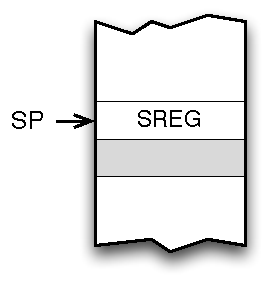
\includegraphics[scale=.6]{pictures/avr8-StackAfterSC.pdf} 
%\end{minipage}
%\begin{minipage}{0.5\textwidth}
%   \caption{Process stack mapping at the beginning of the \texttt{tpl_sc_handler} function. The grayed zone represents an unknown content depending on from where the service was called.}\label{fig:avr8StartTplScHandler}
%\end{minipage}
%\end{figure}

\subsection{Dispatching the service call}

\cfunction{tpl_sc_handler} performs the following tasks:
\begin{penum}
\item save working registers
\item switch to kernel stack if needed
\item calls the service / counter call / ISR
\item performs a context switch if needed
\item switches back to the process stack if needed
\item restore working registers and get back to the process
\end{penum}

\subsubsection{Save working registers}
Some working registers are saved on the user stack. TODO: use volatile registers…

\subsubsection{Switching to the kernel stack}
The first objective of the \cfunction{tpl_sc_handler} is to switch to a kernel stack. However the kernel stack could used already because a call to a \cfunction{PreTaskHook} or a \cfunction{PostTaskHook} is done on the kernel stack and such a hook may call a service. So the dispatch layer is reentrant. The number of reentrant calls is counted by the \var{tpl_reentrancy_counter}.For a reentrant call, the same frame is build over the current one. The switch to the kernel stack is done as follow:

\begin{lstlisting}[language=C]
	//tpl_reentrancy_counter++
	lds r30,tpl_reentrancy_counter //load
	subi r30, 0xFF //r30 <- R30-(-1)
	sts tpl_reentrancy_counter,r30 //store
	//tpl_reentrancy_counter == 1?
	cpi r30,0x01 // compare with immediat
	brne tpl_enter_kernel_end //branch if not equal
	//yes => tpl_switch_to_kernel_stack
	call tpl_switch_to_kernel_stack ;use r2-r6,r30-r31
\end{lstlisting}

When the \cfunction{tpl_switch_to_kernel_stack} returns, SP points to the kernel stack and the stack is empty (figure \ref{fig:avr8kernStackInit}
\begin{figure}[htbp] %  figure placement: here, top, bottom, or page
\begin{minipage}{0.5\textwidth}
    \centering
  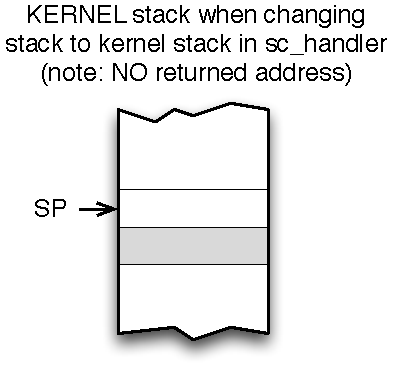
\includegraphics[scale=.6]{pictures/avr8-kernStackInit.pdf} 
\end{minipage}
\begin{minipage}{0.5\textwidth}
   \caption{Kernel stack just after the \cfunction{tpl_switch_to_kernel_stack} function. The grayed zone represents stack bottom.}
   \label{fig:avr8kernStackInit}
\end{minipage}
\end{figure}



Ce qui est fait:
Remanier le fichier tpl_os.c pour:
* le couper en 2 dans les templates
* faire la partie en C directement. Mettre la partie commune de changement de pile directement dans
machine/avr.

il faut rajouter en début de fichier tpl_os.c
\begin{lstlisting}[language=C]
#include <avr/io.h>
#include <avr/interrupt.h>
extern uint8_t tpl_reentrancy_counter;
extern void tpl_switch_to_kernel_stack();
extern void tpl_switch_to_user_stack();
\end{lstlisting}




\subsection{Context}
The context of the AVR is composed of:
\begin{itemize}
\item the stack pointer \texttt{sp}
\item the program counter \texttt{PC}
\item the status register \texttt{SREG} and 
\item 32 GPRs \texttt{r0} to \texttt{r31}. This includes the 3 16-bits indirect registers \texttt{X}, \texttt{Y} and \texttt{Z} which are mapped on these GPRs.
\end{itemize}

However, the context switch uses the stack to save all theses registers (except \texttt{sp} obviously) and the context does not use any structure to save only one variable (SP):
\begin{lstlisting}[language=C]
typedef u16 avr_context;
typedef avr_context *tpl_context;
\end{lstlisting}

Moreover, it is not necessary to save all registers. The ABI impose only to save \texttt{call-Saved Registers}\footnote{see more information on the AVR ABI at \url{https://gcc.gnu.org/wiki/avr-gcc\#Register\_Layout}}. Only \texttt{R2-R17}, \texttt{R28} and \texttt{R29} should be preserved. We also store the status register \texttt{SREG} to allow interrupts at the beginning of tasks (the \texttt{I} flag of \texttt{SREG} is set in \texttt{tpl_init_context}).

\subsection{Context switch}
The context switch implementation uses intensively the stack. The two functions for context switches point to the same code:

\begin{lstlisting}[language=C]
void tpl_switch_context(tpl_context *old, tpl_context *new);
void tpl_switch_context_from_it(tpl_context *old, tpl_context *new);
\end{lstlisting}

\begin{itemize}
\item save the current context (if \texttt{old} is not \texttt{NULL});
\item restore the context from \texttt{new}
\end{itemize}

registers are pushed on the stack like in figure \ref{fig:avr8-stackSave}. The \texttt{GPR} \texttt{r16} is used during the context switch and is the first on the stack. Then, the status register is saved, and all the remaining registers that should be preserved in the ABI. Note that we use the standard \texttt{gcc} frame in interrupts; this frame store all the remaining registers.

\begin{figure}[htbp] %  figure placement: here, top, bottom, or page
\begin{minipage}{0.4\textwidth}
    \centering
  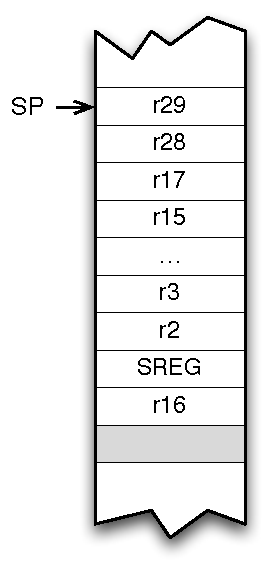
\includegraphics[scale=.6]{pictures/avr8-stackSave.pdf} 
\end{minipage}
\begin{minipage}{0.6\textwidth}
  \caption{Stack of the old_context at the end of context switch}\label{fig:avr8-stackSave}
\end{minipage}
\end{figure}

The restoration of the new context just gets the new stack pointer from the argument \texttt{tpl_context} and pops all these registers.

\subsection{Context init}
The initialization of the context init (\cfunction{tpl_init_context})the stack according to be compliant with the context switch. 

\warning{All the AVR8 do not have the same size of the program counter!! Most of them use a 16-bit program counter, while a few ATMega use a 24-bit program counter!! (if there is more than 64ko of program flash).
}

The gcc compiler defines either the symbol \texttt{\_\_AVR\_3\_BYTE\_PC\_\_} or \texttt{\_\_AVR\_2\_BYTE\_PC\_\_}, which is used in the \texttt{tpl\_machine.c} file.
So, the AVR kind should be defined:

The stack at the end of context init should be like in figure \ref{fig:avr8-stackInit}:
\begin{itemize}
\item The \cfunction{TerminateTask} or \cfunction{CallTerminateISR2} is pushed, depending on the type of the process (task or ISR2)
\item the PC of the entry point of the process is pushed
\item the rest of the context is pushed. All required GPRs are init to \texttt{0x0}, and the status register \texttt{SREG} to \texttt{0x80} to enable interrupts (\texttt{I} bit).
\end{itemize}
\begin{figure}[htbp] %  figure placement: here, top, bottom, or page
\begin{minipage}{0.4\textwidth}
    \centering
  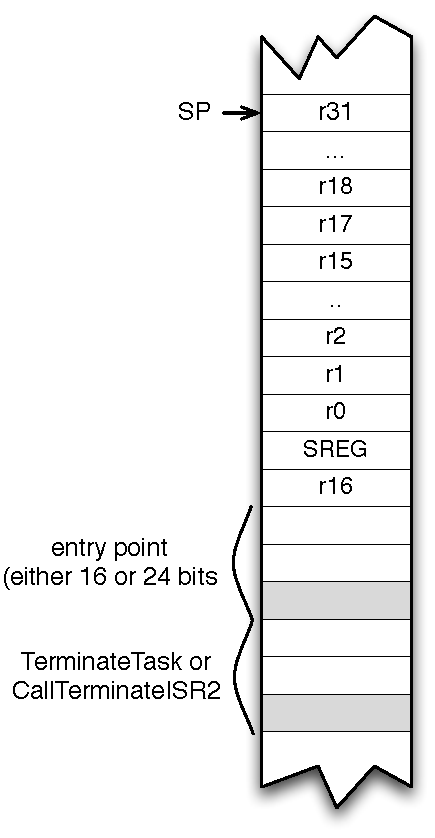
\includegraphics[scale=.6]{pictures/avr8-stackInit.pdf} 
\end{minipage}
\begin{minipage}{0.6\textwidth}
  \caption{Stack at the end of contact init}\label{fig:avr8-stackInit}
\end{minipage}
\end{figure}

\subsection{Interrupts}
Interrupts are handled directly using the standard way by the compiler \texttt{GCC}. \texttt{GCC} saves all the required registers, which are restored at the end of the interrupt.

It should be noted that \texttt{GCC} uses the \texttt{ISR} macro to define an interrupt handler, which is in conflict with the \texttt{ISR} macro defined in Trampoline.

\begin{lstlisting}[language=C]
//gcc uses ISR as a keyword to define an interrupt handler.
//Osek uses ISR to define an ISR2 :-/
#ifdef ISR
 #undef ISR
#endif
#include <avr/interrupt.h>

ISR(TIMER2_OVF_vect)
{

  tpl_counter_tick(&SystemCounter_counter_desc);

  if (tpl_kern.need_schedule)
  {
    tpl_schedule_from_running();
    LOCAL_SWITCH_CONTEXT()
  }
}	
\end{lstlisting}

\section{Arduino Port}
The Arduino port aims to use the Arduino libraries with trampoline on Arduino\footnote{\url{http://www.arduino.cc/}} AVR cards (first targets are Arduino Uno and Arduino Mega).

Arduino libraries have been set in the directory \texttt{machines/avr/arduino} and adapted to Trampoline. They are extracted from the GitHub version (see file machines/avr/arduino/version.txt). Current version is \texttt{1.5.8}.

Some adaptations on libraries should be done, and are explained in the next sections. For an easiest merge with next Arduino libraries, the code modification are well identified with comments:

\begin{lstlisting}[language=C]
// START TRAMPOLINE SECTION 
	void trampolineSystemCounter();
// STOP TRAMPOLINE SECTION 
\end{lstlisting}

Code parts that are removed are also documented:
\begin{lstlisting}[language=C]
// START REMOVE TRAMPOLINE SECTION
	void trampolineSystemCounter();
// STOP REMOVE TRAMPOLINE SECTION
\end{lstlisting}

\subsection{Main adaptation}
In the Arduino approach, the \texttt{main.cpp} file is hidden, and 2 functions should be user defined:
\begin{itemize}
\item \texttt{setup()} initialize the system;
\item \texttt{loop()} is repeated indefinitely;
\end{itemize}

With Trampoline, the \texttt{loop()} function disappears and the \texttt{StartOS()} service should be called at the end of the setup().

To be compliant with the Arduino approach, the \texttt{main.cpp} is hidden in user projects (but is present in \texttt{machines/avr/arduino/main.cpp}. It initializes timers, call the \texttt{setup()} user init function and start the OS with \texttt{StartOS()}. 

Another service is provided to support different application modes\footnote{By default, the application mode \texttt{OSDEFAULTAPPMODE} is used}. The application mode should be defined \emph{during the \texttt{setup()} function}:
\begin{lstlisting}[language=C]
void SetAppMode(AppModeType appMode);
\end{lstlisting}


\subsection{Goil adaptation}
A dedicated section for Arduino is provided in  \texttt{CPU.OS}:
\begin{lstlisting}[language=OIL]
CPU test {    
  OS config {
    ARDUINO = TRUE {
      BOARD = UNO;
      PORT = "/dev/tty.usbmodem1411";
      AVR_LIBC = "/usr/local/CrossPack-AVR/avr/include/";
      SERIAL = TRUE;
    };
    //...
  }
}
\end{lstlisting}

Parameters are:
\begin{description}
\item[\texttt{BOARD}] The Arduino specific board. It should be only \texttt{UNO} or \texttt{MEGA} at this date;
\item[\texttt{PORT}] This is the device associated to the board to flash the AVR, like in the Arduino IDE. On Linux systems it should something like \texttt{/dev/ttyUSB0}.
\item[\texttt{AVR\_LIBC}] This is the place where is the \texttt{libc} for \texttt{avr-gcc}. This is required to get the \texttt{avr/io.h} include file. On Debian/Ubuntu, it should be located in \texttt{"/usr/lib/avr/include"}
\item[\textit{feature}] Add the required files in the project. Current features\footnote{See up-to-date features in Goil specific templates in \texttt{<goilTemplatesDir>/config/avr/arduino/config.oil}} are:
\begin{itemize}
%\item \texttt{SPI}
%\item \texttt{I2C}
%\item \texttt{SERVO}
\item \texttt{SERIAL}
%\item \texttt{NRF24}
%\item \texttt{TINYRTC}
%\item \texttt{TIME}
%\item \texttt{STANDARDWIRING}
%\item \texttt{EVOLVEARDUINO}
%\item \texttt{LCDCRYSTAL}
%\item \texttt{STEPPER}
\end{itemize}
\end{description}

\subsection{System Counter}
The Arduino libraries comes with a SysTick associated to \texttt{TIMER0} interrupt. \texttt{Timer0} has a prescaler factor of 64, and the sysTick period is \textbf{$1024\mu s$} on a 16MHz chip.

The \texttt{SystemCounter} counter is automatically defined\footnote{see file \texttt{<goilTemplatesDir>/config/avr/arduino/config.oil}} and connected to that Arduino \texttt{SysTick}, with:
\begin{itemize}
\item \texttt{TICKSPERBASE = 1}
\item \texttt{MAXALLOWEDVALUE = 65535}
\item \texttt{MINCYCLE = 1}
\end{itemize}

\textbf{This means that the System Counter is hardwired to a 1024 $\mu s$ period}.

The period of this timer cannot be changed has it is used for both Arduino SysTick, and PWM. If you need another resolution, the best way is to use another timer associated to another OSEK counter.
